\section{译者补充:微面模型相关推导}\label{sec:译者补充:微面模型相关推导}
\begin{remark}
    本节内容不是原书内容,而是译者根据\citet{heitz:hal-01024289}和\citet{10.5555/2383847.2383874}整理
    并推导后补充的,请酌情参考和斧正。
\end{remark}
\subsection{微面分布函数的定义与性质}\label{sub:微面分布函数的定义与性质}
如\reffig{08ex01-macrosurfaceMicrosurface},我们考虑一个足够小的宏曲面$\mathcal{G}$,设它是个绝对光滑的平面,具有法线$\bm n$.
微面模型中,真正粗糙起伏的曲面,即微曲面$\mathcal{M}$,是由许多偏离宏曲面的微面构成的。
或者说,微曲面$\mathcal{M}$上所有的点在方向$\bm n$上投影即得$\mathcal{G}$.
将宏曲面上的点记为${\bm p}_{\mathrm{g}}$,其周围的微分面元为$\mathrm{d}{\bm p}_{\mathrm{g}}$,
则宏曲面的面积为
\begin{align}
    S=\int\limits_{\mathcal{G}}\mathrm{d}{\bm p}_{\mathrm{g}}\, .
\end{align}

将$\mathcal{M}$上的点记作${\bm p}_{\mathrm{h}}$,该点处的法线记作${\bm\omega}_{\mathrm{h}}({\bm p}_{\mathrm{h}})$.
引入三维意义下的狄拉克$\delta$分布,
它满足$\displaystyle\int\limits_{\varOmega}\delta({\bm\omega})\mathrm{d}{\bm\omega}=1$.
并记$\delta_{\bm\omega}({\bm\omega}')=\delta({\bm\omega}'-{\bm\omega})$.
由此定义\keyindex{微面分布函数}{microfacet distribution function}{distribution分布}为
\sidenote{原论文全文假定$S=1$来讨论,不用除以面积,这里笔者的处理有所不同。}
\begin{align}\label{eq:08ex01-MicrosurfaceDistribution}
    D({\bm\omega})=\displaystyle\frac{1}{S}\int\limits_{\mathcal{M}}
    \delta_{\bm\omega}({\bm\omega}_{\mathrm{h}}({\bm p}_{\mathrm{h}}))
    \mathrm{d}{\bm p}_{\mathrm{h}}\, ,
\end{align}
其中狄拉克$\delta$分布和$D({\bm\omega}_{\mathrm{h}})$的量纲均为
球面度的倒数即$\displaystyle\frac{1}{\text{sr}}$,也相当于无量纲。

\begin{figure}[htbp]
    \centering
    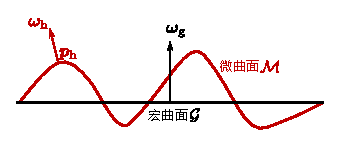
\includegraphics[width=0.6\linewidth]{Pictures/chap08/macrosurfaceMicrosurface.eps}
    \caption{宏曲面(黑色)与微曲面(红色)。}
    \label{fig:08ex01-macrosurfaceMicrosurface}
\end{figure}

我们可以把${\bm\omega}_{\mathrm{h}}$视作从$\mathcal{M}$到整个方向空间$\varOmega$的映射。
注意$\varOmega$包含了球心到完整球面上任意一点的所有可能方向(总立体角为$4\pi$,尽管该映射不一定能覆盖全)。
现在考虑$\mathcal{M}$和$\varOmega$各自的子集$\mathcal{M'}$和$\varOmega'$,
并设它们满足以下条件:点${\bm p}_{\mathrm{h}}$属于$\mathcal{M'}$当且仅当
该点处的微面法线${\bm\omega}_{\mathrm{h}}({\bm p}_{\mathrm{h}})$属于$\varOmega'$,即
\begin{align}
    {\bm p}_{\mathrm{h}}\in\mathcal{M'}\Leftrightarrow
    {\bm\omega}_{\mathrm{h}}({\bm p}_{\mathrm{h}})\in\varOmega'\, .
\end{align}
由此利用积分换元可得微面分布函数具有计算指定微曲面面积的能力:
\begin{align}
    \label{eq:08ex01-microsurfaceArea}
    \int\limits_{\mathcal{M}'}\mathrm{d}{\bm p}_{\mathrm{h}}
    =S\int\limits_{\varOmega'}D({\bm\omega}_{\mathrm{h}})\mathrm{d}{\bm\omega}_{\mathrm{h}}\, .
\end{align}
而整个微曲面面积就是
\begin{align}
    \int\limits_{\mathcal{M}}\mathrm{d}{\bm p}_{\mathrm{h}}
    =S\int\limits_{\varOmega}D({\bm\omega}_{\mathrm{h}})\mathrm{d}{\bm\omega}_{\mathrm{h}}\, .
\end{align}

进一步地,对于任意关于微面法线的函数$f({\bm\omega}_{\mathrm{h}})$,
利用$D({\bm\omega}_{\mathrm{h}})$可将空间积分与统计积分相互转化:
\begin{align}
    \int\limits_{\mathcal{M}}f({\bm\omega}_{\mathrm{h}}({\bm p}_{\mathrm{h}}))\mathrm{d}{\bm p}_{\mathrm{h}}
    =S\int\limits_{\varOmega}f({\bm\omega}_{\mathrm{h}})
    D({\bm\omega}_{\mathrm{h}})\mathrm{d}{\bm\omega}_{\mathrm{h}}\, .
\end{align}

反之,对于任意定义在$\mathcal{M}$上的函数$g({\bm p}_{\mathrm{h}})$,
我们可以定义对应的统计函数$g({\bm\omega}_{\mathrm{h}})$为
\sidenote{这里原论文为了在记号上强调二者的联系,仍然使用了符号$g$,
    但读者应明白这是一个新的函数了。后面\refeq{08ex01-StaticMaskFunc}等的情况类似。}:
\begin{align}\label{eq:08ex01-StaticFunc}
    g({\bm\omega})=\frac{\displaystyle\int\limits_{\mathcal{M}}
    \delta_{\bm\omega}({\bm\omega}_{\mathrm{h}}({\bm p}_{\mathrm{h}}))
    g({\bm p}_{\mathrm{h}})\mathrm{d}{\bm p}_{\mathrm{h}}}
    {\displaystyle\int\limits_{\mathcal{M}}
    \delta_{\bm\omega}({\bm\omega}_{\mathrm{h}}({\bm p}_{\mathrm{h}}))
    \mathrm{d}{\bm p}_{\mathrm{h}}}\, .
\end{align}
该函数也可以实现空间积分与统计积分的相互转化:
\begin{align}\label{eq:08ex01-TransferSpaceStatic}
    \int\limits_{\mathcal{M}}g({\bm p}_{\mathrm{h}})\mathrm{d}{\bm p}_{\mathrm{h}}
    =S\int\limits_{\varOmega}g({\bm\omega}_{\mathrm{h}})
    D({\bm\omega}_{\mathrm{h}})\mathrm{d}{\bm\omega}_{\mathrm{h}}\, .
\end{align}

如\reffig{08ex01-ProjectionsMicrofacetArea},理解以上推导后,我们可以计算以下面积。
\begin{figure}[htbp]
    \centering
    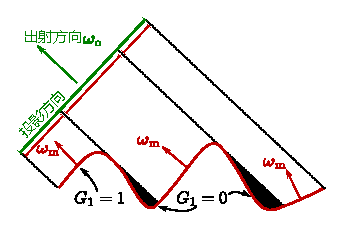
\includegraphics[width=0.5\linewidth]{Pictures/chap08/ProjectionsMicrofacet.eps}
    \caption{微面可见部分在${\bm\omega}_{\mathrm{o}}$上的投影面积。}
    \label{fig:08ex01-ProjectionsMicrofacetArea}
\end{figure}

首先,微曲面在宏曲面法线方向${\bm\omega}_{\mathrm{g}}$上的
投影面积(不论是否遮挡,且背向时记负值)为
\begin{align}
    \int\limits_{\mathcal{M}}({\bm\omega}_{\mathrm{h}}({\bm p}_{\mathrm{h}})
    \cdot{\bm\omega}_{\mathrm{g}})\mathrm{d}{\bm p}_{\mathrm{h}}
    =S\int\limits_{\varOmega}({\bm\omega}_{\mathrm{h}}\cdot{\bm\omega}_{\mathrm{g}})
    D({\bm\omega}_{\mathrm{h}})\mathrm{d}{\bm\omega}_{\mathrm{h}}
    =\int\limits_{\mathcal{G}}\mathrm{d}{\bm p}_{\mathrm{g}}=S\, .
\end{align}
注意上式同时给出了一个$D({\bm\omega}_{\mathrm{h}})$应满足的重要约束:
\begin{align}\label{eq:08ex01-McrofacetDistributionNormalization}
    \int\limits_{\varOmega}({\bm\omega}_{\mathrm{h}}\cdot{\bm\omega}_{\mathrm{g}})
    D({\bm\omega}_{\mathrm{h}})\mathrm{d}{\bm\omega}_{\mathrm{h}}=1\, .
\end{align}

接着我们从出射方向${\bm\omega}_{\mathrm{o}}$来观察曲面。此时宏曲面在${\bm\omega}_{\mathrm{o}}$上的投影面积为
\begin{align}
    \label{eq:08ex01-AreaMacrosurface}
    ({\bm\omega}_{\mathrm{o}}\cdot{\bm\omega}_{\mathrm{g}})S=S\cos\theta_{\mathrm{o}}\, ,
\end{align}
其中$\theta_{\mathrm{o}}$为${\bm\omega}_{\mathrm{o}}$与${\bm\omega}_{\mathrm{g}}$的夹角。

最后我们算得微面可见部分在${\bm\omega}_{\mathrm{o}}$上的投影面积为
\begin{align}\label{eq:08ex01-AreaProjectionsMicrofacetVisible}
    \int\limits_{\mathcal{M}}G_1({\bm p}_{\mathrm{h}},{\bm\omega}_{\mathrm{o}})
    \max({\bm\omega}_{\mathrm{h}}({\bm p}_{\mathrm{h}})\cdot{\bm\omega}_{\mathrm{o}},0)
    \mathrm{d}{\bm p}_{\mathrm{h}}\, ,
\end{align}
其中\keyindex{空间掩模函数}{spatial masking function}{masking function掩模函数}
$G_1({\bm p}_{\mathrm{h}},{\bm\omega}_{\mathrm{o}})$在${\bm p}_{\mathrm{h}}$被
遮挡时取0,否则取1. 而$\max$项则过滤了背向不可见的微面。
其对应的\keyindex{统计掩模函数}{statistical masking function}{masking function掩模函数}
$G_1({\bm\omega}_{\mathrm{h}},{\bm\omega}_{\mathrm{o}})$的值域为$[0,1]$,
它给出了从方向${\bm\omega}_{\mathrm{o}}$观察时,法线为${\bm\omega}_{\mathrm{h}}$的微面中可见的比例:
\begin{align}\label{eq:08ex01-StaticMaskFunc}
    G_1({\bm\omega},{\bm\omega}_{\mathrm{o}})
    =\frac{\displaystyle\int\limits_{\mathcal{M}}
    \delta_{\bm\omega}({\bm\omega}_{\mathrm{h}}({\bm p}_{\mathrm{h}}))
    G_1({\bm p}_{\mathrm{h}},{\bm\omega}_{\mathrm{o}})\mathrm{d}{\bm p}_{\mathrm{h}}}
    {\displaystyle\int\limits_{\mathcal{M}}
    \delta_{\bm\omega}({\bm\omega}_{\mathrm{h}}({\bm p}_{\mathrm{h}}))
    \mathrm{d}{\bm p}_{\mathrm{h}}}\, .
\end{align}
由此得到投影面积的另一计算方式:
\begin{align}
    \label{eq:08ex01-AreaMicrosurface}
    S\int\limits_{\varOmega}G_1({\bm\omega}_{\mathrm{h}},{\bm\omega}_{\mathrm{o}})
    \max({\bm\omega}_{\mathrm{h}}\cdot{\bm\omega}_{\mathrm{o}},0)
    D({\bm\omega}_{\mathrm{h}})\mathrm{d}{\bm\omega}_{\mathrm{h}}\, .
\end{align}

由于可见微面投影面积等于宏曲面投影面积,所以
结合\refeq{08ex01-AreaMacrosurface}和\refeq{08ex01-AreaMicrosurface}可得
基于物理的掩模函数$G_1$总是满足如下约束:
\begin{align}\label{eq:08ex01-CosThetaO}
    \cos\theta_{\mathrm{o}}=\int\limits_{\varOmega}
    G_1({\bm\omega}_{\mathrm{h}},{\bm\omega}_{\mathrm{o}})
    \max({\bm\omega}_{\mathrm{h}}\cdot{\bm\omega}_{\mathrm{o}},0)
    D({\bm\omega}_{\mathrm{h}})\mathrm{d}{\bm\omega}_{\mathrm{h}}\, .
\end{align}
注意这并不意味着该约束唯一确定了$G_1$,它常常有无数个解。
还需引入其他约束或假设才能限定为唯一解。
\reffig{08ex01-SameDistributionOfNormalsDifferentBRDFs}给出了这种不唯一性的例子。
\begin{figure}[htbp]
    \centering
    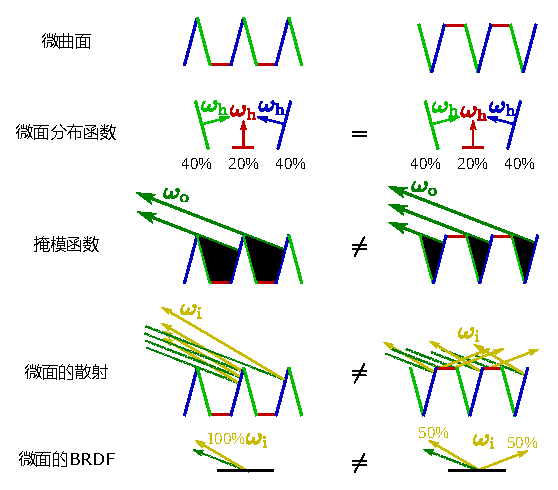
\includegraphics[width=0.75\linewidth]{Pictures/chap08/SameDistributionOfNormalsDifferentBRDFs.eps}
    \caption{具有相同微面分布函数$D({\bm\omega}_{\mathrm{h}})$但BRDF却不同的两种微面。}
    \label{fig:08ex01-SameDistributionOfNormalsDifferentBRDFs}
\end{figure}

此外,译者再补充两个\refeq{08ex01-StaticMaskFunc}可能让人感到困惑的地方:

第一个是记号的问题。$G_1({\bm\omega}_{\mathrm{h}},{\bm\omega}_{\mathrm{o}})$中
第一个自变量是${\bm\omega}_{\mathrm{h}}$,该变量应出现在其定义式中狄拉克$\delta$分布的下标,
但狄拉克$\delta$分布后面的括号内还有一个记号相同的函数${\bm\omega}_{\mathrm{h}}({\bm p}_{\mathrm{h}})$,
所以为了区分它们,\refeq{08ex01-StaticMaskFunc}中临时把第一个自变量改写为${\bm\omega}$.
笔者保留了原论文的这个做法,请读者注意区分。\refeq{08ex01-MicrosurfaceDistribution}、
\refeq{08ex01-StaticFunc}和\refeq{08ex01-AnotherStaticFunc}也用了类似的临时记号。

第二个是定义的问题。细心的读者可能注意到,
比对\refeq{08ex01-AreaProjectionsMicrofacetVisible}和\refeq{08ex01-TransferSpaceStatic},
我们本该设
\begin{align}\label{eq:08ex01-AnotherSpaceFunc}
    g({\bm p}_{\mathrm{h}})=G_1({\bm p}_{\mathrm{h}},{\bm\omega}_{\mathrm{o}})
    \max({\bm\omega}_{\mathrm{h}}({\bm p}_{\mathrm{h}})\cdot{\bm\omega}_{\mathrm{o}},0)\, ,
\end{align}
此时使得\refeq{08ex01-TransferSpaceStatic}成立的$g({\bm\omega}_{\mathrm{h}})$应该是
把\refeq{08ex01-AnotherSpaceFunc}带入\refeq{08ex01-StaticFunc}得到的
\begin{align}\label{eq:08ex01-AnotherStaticFunc}
    g({\bm\omega})=\frac{\displaystyle\int\limits_{\mathcal{M}}
    \delta_{\bm\omega}({\bm\omega}_{\mathrm{h}}({\bm p}_{\mathrm{h}}))
    G_1({\bm p}_{\mathrm{h}},{\bm\omega}_{\mathrm{o}})
    \max({\bm\omega}_{\mathrm{h}}({\bm p}_{\mathrm{h}})\cdot{\bm\omega}_{\mathrm{o}},0)
    \mathrm{d}{\bm p}_{\mathrm{h}}}
    {\displaystyle\int\limits_{\mathcal{M}}
    \delta_{\bm\omega}({\bm\omega}_{\mathrm{h}}({\bm p}_{\mathrm{h}}))
    \mathrm{d}{\bm p}_{\mathrm{h}}}\, .
\end{align}
将上式回代\refeq{08ex01-TransferSpaceStatic}的右边后,
读者会发现它和\refeq{08ex01-AreaMicrosurface}并不是完全一样的——
后者相当于把前者内层积分中的项$\max({\bm\omega}_{\mathrm{h}}({\bm p}_{\mathrm{h}})\cdot{\bm\omega}_{\mathrm{o}},0)$
(里面的${\bm\omega}_{\mathrm{h}}$是函数)提到外层积分中
变成了$\max({\bm\omega}_{\mathrm{h}}\cdot{\bm\omega}_{\mathrm{o}},0)$
(里面的${\bm\omega}_{\mathrm{h}}$是变量)。
一般来说积分变量并不能随便外提,但因为这里内层积分中含有狄拉克$\delta$分布,
它使得此处外提$\max$项的做法恰好没有改变整个式子的值。
所以原论文中作出简化处理,相当于令$g({\bm p}_{\mathrm{h}})=G_1({\bm p}_{\mathrm{h}},{\bm\omega}_{\mathrm{o}})$,
此时对应的$g({\bm\omega}_{\mathrm{h}})$即为\refeq{08ex01-StaticMaskFunc}中
的$G_1({\bm\omega}_{\mathrm{h}},{\bm\omega}_{\mathrm{o}})$.
不过原作者并未交代这样的细节。后面\refeq{08ex01-RadianceMicrofacet}也用了类似技巧。

\subsection{基于微面模型的BRDF}\label{sub:基于微面模型的BRDF}
本节继承上节的记号。在微面尺度上,我们设微面上一点朝出射方向${\bm\omega}_{\mathrm{o}}$的辐亮度
为$L_{\mathcal{M}}({\bm\omega}_{\mathrm{h}}({\bm p}_{\mathrm{h}}),{\bm\omega}_{\mathrm{o}})$.
则从宏观尺度看,该微面整体朝${\bm\omega}_{\mathrm{o}}$等价的出射
辐亮度$L_{\mathrm{o}}({\bm\omega}_{\mathrm{o}})$即为
微面尺度的辐亮度按出射方向可见投影面积比例的加权:
\begin{align}\label{eq:08ex01-RadianceMicrofacetAverageSum}
    L_{\mathrm{o}}({\bm\omega}_{\mathrm{o}})
    =\frac{\displaystyle\int\limits_{\mathcal{M}}
    {L_{\mathcal{M}}({\bm\omega}_{\mathrm{h}}({\bm p}_{\mathrm{h}}),{\bm\omega}_{\mathrm{o}})
    G_1({\bm p}_{\mathrm{h}},{\bm\omega}_{\mathrm{o}})
    \max({\bm\omega}_{\mathrm{h}}({\bm p}_{\mathrm{h}})\cdot{\bm\omega}_{\mathrm{o}},0)
    \mathrm{d}{\bm p}_{\mathrm{h}}}}
    {\displaystyle\int\limits_{\mathcal{M}}
    {G_1({\bm p}_{\mathrm{h}},{\bm\omega}_{\mathrm{o}})
    \max({\bm\omega}_{\mathrm{h}}({\bm p}_{\mathrm{h}})\cdot{\bm\omega}_{\mathrm{o}},0)
    \mathrm{d}{\bm p}_{\mathrm{h}}}}\, .
\end{align}
上式利用空间掩模函数\refeq{08ex01-StaticMaskFunc}转化为统计积分形式,
并将\refeq{08ex01-AreaProjectionsMicrofacetVisible}带入分母可得:
\begin{align}\label{eq:08ex01-RadianceMicrofacet}
    L_{\mathrm{o}}({\bm\omega}_{\mathrm{o}})
    =\frac{1}{\cos\theta_{\mathrm{o}}}\int\limits_{\varOmega}
    L_{\mathcal{M}}({\bm\omega}_{\mathrm{h}},{\bm\omega}_{\mathrm{o}})
    G_1({\bm\omega}_{\mathrm{h}},{\bm\omega}_{\mathrm{o}})
    \max({\bm\omega}_{\mathrm{h}}\cdot{\bm\omega}_{\mathrm{o}},0)
    D({\bm\omega}_{\mathrm{h}})\mathrm{d}{\bm\omega}_{\mathrm{h}}\, .
\end{align}
观察上式,我们把被积分项中对$L_{\mathcal{M}}({\bm\omega}_{\mathrm{h}},{\bm\omega}_{\mathrm{o}})$加权的系数
定义为\keyindex{可见法线分布}{distribution of visible normals}{distribution分布}:
\begin{align}\label{eq:08ex01-DistributionOfVisibleNormals}
    D_{{\bm\omega}_{\mathrm{o}}}({\bm\omega}_{\mathrm{h}})
    =\frac{G_1({\bm\omega}_{\mathrm{h}},{\bm\omega}_{\mathrm{o}})
        \max({\bm\omega}_{\mathrm{h}}\cdot{\bm\omega}_{\mathrm{o}},0)
        D({\bm\omega}_{\mathrm{h}})}{\cos\theta_{\mathrm{o}}}\, .
\end{align}
其中$\cos\theta_{\mathrm{o}}$如\refeq{08ex01-AreaMacrosurface}所述
即${\bm\omega}_{\mathrm{o}}\cdot{\bm\omega}_{\mathrm{g}}$,
于是\refeq{08ex01-RadianceMicrofacet}可以表示为:
\begin{align}\label{eq:08ex01-RadianceMacroOut}
    L_{\mathrm{o}}({\bm\omega}_{\mathrm{o}})
    =\int\limits_{\varOmega}L_{\mathcal{M}}({\bm\omega}_{\mathrm{h}},{\bm\omega}_{\mathrm{o}})
    D_{{\bm\omega}_{\mathrm{o}}}({\bm\omega}_{\mathrm{h}})\mathrm{d}{\bm\omega}_{\mathrm{h}}\, .
\end{align}
同时应注意到该定义下$D_{{\bm\omega}_{\mathrm{o}}}({\bm\omega}_{\mathrm{h}})$满足规范化性质:
\begin{align}\label{eq:08ex01-VisibleDistributionNormalization}
    \int\limits_{\varOmega}D_{{\bm\omega}_{\mathrm{o}}}({\bm\omega}_{\mathrm{h}})
    \mathrm{d}{\bm\omega}_{\mathrm{h}}=1\, .
\end{align}
若再结合\refeq{08ex01-CosThetaO},则$L_{\mathrm{o}}({\bm\omega}_{\mathrm{o}})$还可以表示为以下形式:
\begin{align}\label{eq:08ex01-RadianceMacroOutV2}
    L_{\mathrm{o}}({\bm\omega}_{\mathrm{o}})
    =\frac{\displaystyle\int\limits_{\varOmega}L_{\mathcal{M}}({\bm\omega}_{\mathrm{h}},{\bm\omega}_{\mathrm{o}})
    G_1({\bm\omega}_{\mathrm{h}},{\bm\omega}_{\mathrm{o}})
    \max({\bm\omega}_{\mathrm{h}}\cdot{\bm\omega}_{\mathrm{o}},0)
    D({\bm\omega}_{\mathrm{h}})\mathrm{d}{\bm\omega}_{\mathrm{h}}}
    {\displaystyle\int\limits_{\varOmega}G_1({\bm\omega}_{\mathrm{h}},{\bm\omega}_{\mathrm{o}})
    \max({\bm\omega}_{\mathrm{h}}\cdot{\bm\omega}_{\mathrm{o}},0)
    D({\bm\omega}_{\mathrm{h}})\mathrm{d}{\bm\omega}_{\mathrm{h}}}\, .
\end{align}

接下来我们利用微面尺度上的BRDF推导微面模型在宏观尺度下的BRDF。
把微面尺度上的BRDF记作$f_{\mathcal{M}}({\bm\omega}_{\mathrm{h}},{\bm\omega}_{\mathrm{o}},{\bm\omega}_{\mathrm{i}})$,
考虑到有效的角度范围,则根据\refeq{5.8}中BRDF的定义有
\begin{align}\label{eq:08ex01-MicrosurfaceBRDF}
    f_{\mathcal{M}}({\bm\omega}_{\mathrm{h}},{\bm\omega}_{\mathrm{o}},{\bm\omega}_{\mathrm{i}})
    =\frac{\mathrm{d} L_{\mathcal{M}}({\bm\omega}_{\mathrm{h}},{\bm\omega}_{\mathrm{o}})}
    {\max({\bm\omega}_{\mathrm{h}}\cdot{\bm\omega}_{\mathrm{i}},0)
    L_{\mathrm{i}}({\bm\omega}_{\mathrm{i}})\mathrm{d}{\bm\omega}_{\mathrm{i}}}\, ,
\end{align}
其中$L_{\mathrm{i}}({\bm\omega}_{\mathrm{i}})$是来自入射方向${\bm\omega}_{\mathrm{i}}$的辐亮度。
由此我们根据定义并结合\refeq{08ex01-RadianceMacroOut}、\refeq{08ex01-MicrosurfaceBRDF}、
\refeq{08ex01-DistributionOfVisibleNormals}得到宏观尺度下的BRDF为:
\begin{align}\label{eq:08ex01-MacroBRDFG1}
    f_{\mathrm{r}}({\bm\omega}_{\mathrm{o}},{\bm\omega}_{\mathrm{i}})
     & = \frac{\mathrm{d} L_{\mathrm{o}}({\bm\omega}_{\mathrm{o}})}
    {|{\bm\omega}_{\mathrm{g}}\cdot{\bm\omega}_{\mathrm{i}}|
    L_{\mathrm{i}}({\bm\omega}_{\mathrm{i}})\mathrm{d}{\bm\omega}_{\mathrm{i}}}
    = \frac{1}{|{\bm\omega}_{\mathrm{g}}\cdot{\bm\omega}_{\mathrm{i}}|}
    \int\limits_{\varOmega}\frac{\mathrm{d}L_{\mathcal{M}}({\bm\omega}_{\mathrm{h}},{\bm\omega}_{\mathrm{o}})}
    {L_{\mathrm{i}}({\bm\omega}_{\mathrm{i}})\mathrm{d}{\bm\omega}_{\mathrm{i}}}
    D_{{\bm\omega}_{\mathrm{o}}}({\bm\omega}_{\mathrm{h}})\mathrm{d}{\bm\omega}_{\mathrm{h}}\nonumber \\
     & = \frac{1}{|{\bm\omega}_{\mathrm{g}}\cdot{\bm\omega}_{\mathrm{i}}|}
    \int\limits_{\varOmega}f_{\mathcal{M}}({\bm\omega}_{\mathrm{h}},{\bm\omega}_{\mathrm{o}},{\bm\omega}_{\mathrm{i}})
    \max({\bm\omega}_{\mathrm{h}}\cdot{\bm\omega}_{\mathrm{i}},0)
    D_{{\bm\omega}_{\mathrm{o}}}({\bm\omega}_{\mathrm{h}})\mathrm{d}{\bm\omega}_{\mathrm{h}}\nonumber \\
     & = \frac{1}{|{\bm\omega}_{\mathrm{g}}\cdot{\bm\omega}_{\mathrm{i}}|
    |{\bm\omega}_{\mathrm{g}}\cdot{\bm\omega}_{\mathrm{o}}|}
    \int\limits_{\varOmega}f_{\mathcal{M}}({\bm\omega}_{\mathrm{h}},{\bm\omega}_{\mathrm{o}},{\bm\omega}_{\mathrm{i}})
    \max({\bm\omega}_{\mathrm{h}}\cdot{\bm\omega}_{\mathrm{i}},0)\nonumber                            \\
     & \qquad\qquad\max({\bm\omega}_{\mathrm{h}}\cdot{\bm\omega}_{\mathrm{o}},0)
    G_1({\bm\omega}_{\mathrm{h}},{\bm\omega}_{\mathrm{o}})
    D({\bm\omega}_{\mathrm{h}})\mathrm{d}{\bm\omega}_{\mathrm{h}}\, .
\end{align}

我们应注意到,上式考虑的其实是入射光在曲面上经历第一次反射后刚刚离开的情形,
并未考虑到反射的光线可能还会再命中曲面一次甚至多次然后从其他方向射出的情况。
然而我们在宏观尺度下的BRDF是定义在单次反射的情形下的,所以应排除掉这些光线。
为此,我们引入\keyindex{遮挡函数}{shadowing function}{}来到达这一效果。
实际中,我们通常直接使用联合的\keyindex{掩模遮挡函数}{masking-shadowing function}{}$G_2$来代替$G_1$,
它计入的微面比例要求在${\bm\omega}_{\mathrm{o}}$和${\bm\omega}_{\mathrm{i}}$上双向可见,此时
\begin{align}\label{eq:08ex01-MacroBRDFG2}
    f_{\mathrm{r}}({\bm\omega}_{\mathrm{o}},{\bm\omega}_{\mathrm{i}})
     & =\frac{1}{|{\bm\omega}_{\mathrm{g}}\cdot{\bm\omega}_{\mathrm{i}}||{\bm\omega}_{\mathrm{g}}\cdot{\bm\omega}_{\mathrm{o}}|}
    \int\limits_{\varOmega}f_{\mathcal{M}}({\bm\omega}_{\mathrm{h}},{\bm\omega}_{\mathrm{o}},{\bm\omega}_{\mathrm{i}})
    \max({\bm\omega}_{\mathrm{h}}\cdot{\bm\omega}_{\mathrm{i}},0)\nonumber                                                       \\
     & \qquad\qquad\max({\bm\omega}_{\mathrm{h}}\cdot{\bm\omega}_{\mathrm{o}},0)
    G_2({\bm\omega}_{\mathrm{h}},{\bm\omega}_{\mathrm{o}},{\bm\omega}_{\mathrm{i}})
    D({\bm\omega}_{\mathrm{h}})\mathrm{d}{\bm\omega}_{\mathrm{h}}\, .
\end{align}

最后,笔者认为对于透射的情况,将\refeq{08ex01-RadianceMicrofacetAverageSum}、
\refeq{08ex01-RadianceMicrofacet}、
\refeq{08ex01-DistributionOfVisibleNormals}、
\refeq{08ex01-RadianceMacroOutV2}、\refeq{08ex01-MicrosurfaceBRDF}、
\refeq{08ex01-MacroBRDFG1}、\refeq{08ex01-MacroBRDFG2}
中的$\max(\cdot,0)$项均改为对应的绝对值$|\cdot|$即可。

\subsection{镜面微面模型的BRDF}\label{sub:镜面微面模型的BRDF}
本节继承上节的记号。为了算出微面模型在宏观尺度下的BRDF,
即\refeq{08ex01-MacroBRDFG1}或\refeq{08ex01-MacroBRDFG2},
我们需要知道微面尺度下的BRDF即$f_{\mathcal{M}}({\bm\omega}_{\mathrm{h}},{\bm\omega}_{\mathrm{o}},{\bm\omega}_{\mathrm{i}})$的具体形式。
本小节假设微面都遵循完美镜面反射,由此给出具体推导。
设微面镜面的菲涅尔反射率为$F_{\mathcal{M}}({\bm\omega}_{\mathrm{h}},{\bm\omega}_{\mathrm{o}})$,
这意味着微面的入射和出射辐亮度满足约束
\begin{align}\label{eq:08ex01-FresnelMicrofacet}
    L_{\mathcal{M}}({\bm\omega}_{\mathrm{h}},{\bm\omega}_{\mathrm{o}})=F_{\mathcal{M}}({\bm\omega}_{\mathrm{h}},{\bm\omega}_{\mathrm{o}})L_{\mathrm{i}}({\bm\omega}_{\mathrm{i}})\, .
\end{align}
考虑到微面遵循完美镜面反射,只有当入射方向、出射方向、法线三者满足
反射定律\ref{theorem:0607-LawOfReflection}描述的情形时,
反射才实际成立,也即上式才成立,其余情况则不成立。
所以$f_{\mathcal{M}}({\bm\omega}_{\mathrm{h}},{\bm\omega}_{\mathrm{o}},{\bm\omega}_{\mathrm{i}})$应
含有狄拉克$\delta$分布来区分这两种情况。因此我们构造出
\begin{align}\label{eq:08ex01-FresnelBRDFMicrofacet}
    f_{\mathcal{M}}({\bm\omega}_{\mathrm{h}},{\bm\omega}_{\mathrm{o}},{\bm\omega}_{\mathrm{i}})
    =F_{\mathcal{M}}({\bm\omega}_{\mathrm{h}},{\bm\omega}_{\mathrm{o}})\frac{\delta_{{\bm\omega}_{\mathrm{r}}}({\bm\omega}_{\mathrm{i}})}{|{\bm\omega}_{\mathrm{h}}\cdot{\bm\omega}_{\mathrm{i}}|}\, ,
\end{align}
其中${\bm\omega}_{\mathrm{r}}$是由${\bm\omega}_{\mathrm{h}}$和${\bm\omega}_{\mathrm{o}}$确定的
满足完美镜面反射的规范化入射方向,即意味着它是
关于${\bm\omega}_{\mathrm{h}}$和${\bm\omega}_{\mathrm{o}}$的函数。
我们可以验证这个构造在完美镜面反射成立
(即${\bm\omega}_{\mathrm{r}}={\bm\omega}_{\mathrm{i}}$)时是符合\refeq{08ex01-FresnelMicrofacet}的:
联立\refeq{08ex01-MicrosurfaceBRDF},在有效的入射方向范围${\varOmega}_{\mathrm{i}}$内积分可得
\begin{align}\label{eq:08ex01-FresnelBRDFValid}
    L_{\mathcal{M}}({\bm\omega}_{\mathrm{h}},{\bm\omega}_{\mathrm{o}})
     & =\int\limits_{{\varOmega}_{\mathrm{i}}}f_{\mathcal{M}}({\bm\omega}_{\mathrm{h}},{\bm\omega}_{\mathrm{o}},{\bm\omega}'_{\mathrm{i}})
    \max({\bm\omega}_{\mathrm{h}}\cdot{\bm\omega}'_{\mathrm{i}},0)
    L_{\mathrm{i}}({\bm\omega}'_{\mathrm{i}})\mathrm{d}{\bm\omega}'_{\mathrm{i}}\nonumber                                                  \\
     & =\int\limits_{{\varOmega}_{\mathrm{i}}}F_{\mathcal{M}}({\bm\omega}_{\mathrm{h}},{\bm\omega}_{\mathrm{o}})
    \delta_{{\bm\omega}_{\mathrm{r}}}({\bm\omega}'_{\mathrm{i}})
    L_{\mathrm{i}}({\bm\omega}'_{\mathrm{i}})\mathrm{d}{\bm\omega}'_{\mathrm{i}}\nonumber                                                  \\
     & =F_{\mathcal{M}}({\bm\omega}_{\mathrm{h}},{\bm\omega}_{\mathrm{o}})L_{\mathrm{i}}({\bm\omega}_{\mathrm{r}})\nonumber                \\
     & =F_{\mathcal{M}}({\bm\omega}_{\mathrm{h}},{\bm\omega}_{\mathrm{o}})L_{\mathrm{i}}({\bm\omega}_{\mathrm{i}})\, .
\end{align}
其他情况下,则等价于$L_{\mathrm{i}}({\bm\omega}_{\mathrm{r}})=0$,
使得$L_{\mathcal{M}}({\bm\omega}_{\mathrm{h}},{\bm\omega}_{\mathrm{o}})=0$,即无反射。

然而\refeq{08ex01-FresnelBRDFMicrofacet}仍然不方便我们推导微面模型的BRDF,
因为\refeq{08ex01-MacroBRDFG1}、\refeq{08ex01-MacroBRDFG2}都需要
对${\bm\omega}_{\mathrm{h}}$积分,但\refeq{08ex01-FresnelBRDFMicrofacet}中
狄拉克$\delta$分布的角标${\bm\omega}_{\mathrm{r}}$是
代入了${\bm\omega}_{\mathrm{h}}$的函数,${\bm\omega}_{\mathrm{h}}$处在这个位置并不便于计算积分。
因此我们需要在保证前面关于积分的推导(尤其是\refeq{08ex01-FresnelBRDFValid})仍然成立的条件下进行换元。
我们设${\bm\omega}_{\mathrm{m}}$是由${\bm\omega}_{\mathrm{i}}$和${\bm\omega}_{\mathrm{o}}$确定的
满足完美镜面反射的规范化微面法线方向,并设满足完美镜面反射的入射方向与微面法线的映射关系为$\bm P$,即:
\begin{align}
    {\bm P}({\bm\omega}_{\mathrm{m}})={\bm\omega}_{\mathrm{i}}\, , \\
    {\bm P}({\bm\omega}_{\mathrm{h}})={\bm\omega}_{\mathrm{r}}\, .
\end{align}
对$\bm P$作一阶近似并利用定理\ref{theorem:7.ex01.symmetry}的结论,可得
\begin{align}\label{eq:08ex01-DeltaChangeVar}
    \delta_{{\bm\omega}_{\mathrm{r}}}({\bm\omega}_{\mathrm{i}})
     & =\delta({\bm\omega}_{\mathrm{i}}-{\bm\omega}_{\mathrm{r}})
    =\delta({\bm P}({\bm\omega}_{\mathrm{m}})-{\bm P}({\bm\omega}_{\mathrm{h}}))
    =\displaystyle\delta\left(({\bm\omega}_{\mathrm{m}}-{\bm\omega}_{\mathrm{h}})
    \frac{\partial{\bm P}({\bm\omega}_{\mathrm{m}})}{\partial{\bm\omega}_{\mathrm{m}}}\right)\nonumber \\
     & =\displaystyle\delta\left(({\bm\omega}_{\mathrm{m}}-{\bm\omega}_{\mathrm{h}})
    \frac{\partial{\bm\omega}_{\mathrm{i}}}{\partial{\bm\omega}_{\mathrm{m}}}\right)
    =\delta({\bm\omega}_{\mathrm{m}}-{\bm\omega}_{\mathrm{h}})
    \left\lVert\frac{\partial{\bm\omega}_{\mathrm{m}}}{\partial{\bm\omega}_{\mathrm{i}}}\right\rVert
    =\delta_{{\bm\omega}_{\mathrm{m}}}({\bm\omega}_{\mathrm{h}})
    \left\lVert\frac{\partial{\bm\omega}_{\mathrm{m}}}{\partial{\bm\omega}_{\mathrm{i}}}\right\rVert\, .
\end{align}
其中$\displaystyle\frac{\partial{\bm\omega}_{\mathrm{m}}}{\partial{\bm\omega}_{\mathrm{i}}}$是
${\bm\omega}_{\mathrm{m}}$对${\bm\omega}_{\mathrm{i}}$的\keyindex{雅可比矩阵}{Jacobian matrix}{matrix矩阵}。
将其套在里面的两层$|\cdot|$表示先求矩阵的\keyindex{行列式}{determinant}{}再取绝对值。
几何意义上,它表示${\bm\omega}_{\mathrm{m}}$和${\bm\omega}_{\mathrm{i}}$发生扰动时
两者各自扰动范围对应的立体角大小之比。
我们在\reffig{08ex01-JacobianRefraction}中推导求解该比值的方法:
\begin{figure}[htbp]
    \centering
    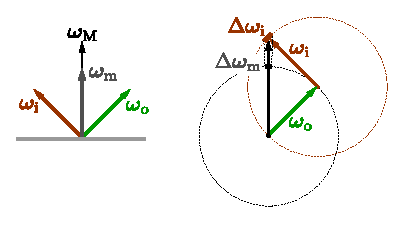
\includegraphics[width=0.6\linewidth]{Pictures/chap08/JacobianRefraction.eps}
    \caption{镜面反射中的角度扰动关系和相应雅可比矩阵行列式绝对值的计算。}
    \label{fig:08ex01-JacobianRefraction}
\end{figure}

将表示入射方向${\bm\omega}_{\mathrm{i}}$和出射方向${\bm\omega}_{\mathrm{o}}$的向量首尾相接。
在完美镜面反射配置下,两者之和必与曲面法线${\bm\omega}_{\mathrm{m}}$共线,因此我们记
\begin{align}
    {\bm\omega}_{\mathrm{M}}=\mathrm{sign}({\bm\omega}_{\mathrm{i}}\cdot{\bm\omega}_{\mathrm{m}})
    \cdot({\bm\omega}_{\mathrm{i}}+{\bm\omega}_{\mathrm{o}})\, ,
\end{align}
其中sign一项是为了将其调整到曲面朝外的方向(和${\bm\omega}_{\mathrm{m}}$同向)
(sign对正数取1,对负数取-1,对零取0);
于是规范化的${\bm\omega}_{\mathrm{m}}$满足
\begin{align}
    {\bm\omega}_{\mathrm{m}}=\frac{{\bm\omega}_{\mathrm{M}}}{|{\bm\omega}_{\mathrm{M}}|}\, .
\end{align}
当${\bm\omega}_{\mathrm{i}}$存在立体角大小为$\Delta{\bm\omega}_{\mathrm{i}}$的微小扰动范围时,
其末端扰动范围的面积是在以${\bm\omega}_{\mathrm{i}}$起点
为球心的单位球表面计算的,大小也为$\Delta{\bm\omega}_{\mathrm{i}}$.
同时它也引发了${\bm\omega}_{\mathrm{m}}$的扰动,
我们即需要计算这块扰动区域对于${\bm\omega}_{\mathrm{m}}$而言是多大的立体角。
回顾定义\ref{definition:SolidAngle},考虑到扰动区域法线
(即${\bm\omega}_{\mathrm{i}}$)和${\bm\omega}_{\mathrm{m}}$存在夹角,
因此它对${\bm\omega}_{\mathrm{m}}$的起点所成的立体角大小$\Delta{\bm\omega}_{\mathrm{m}}$为
\begin{align}
    \Delta{\bm\omega}_{\mathrm{m}}=\frac{|{\bm\omega}_{\mathrm{m}}\cdot{\bm\omega}_{\mathrm{i}}|}
    {|{\bm\omega}_{\mathrm{M}}|^2}\Delta{\bm\omega}_{\mathrm{i}}\, .
\end{align}
同时注意到$|{\bm\omega}_{\mathrm{i}}|=|{\bm\omega}_{\mathrm{o}}|=1$,所以
\begin{align}
    |{\bm\omega}_{\mathrm{M}}|=2|{\bm\omega}_{\mathrm{m}}\cdot{\bm\omega}_{\mathrm{i}}|\, .
\end{align}
于是
\begin{align}\label{eq:08ex01-JacobianRefraction}
    \left\lVert\frac{\partial{\bm\omega}_{\mathrm{m}}}{\partial{\bm\omega}_{\mathrm{i}}}\right\rVert
    =\lim\limits_{\Delta{\bm\omega}_{\mathrm{i}}\to0}\frac{|\Delta{\bm\omega}_{\mathrm{m}}|}{|\Delta{\bm\omega}_{\mathrm{i}}|}
    =\frac{|{\bm\omega}_{\mathrm{m}}\cdot{\bm\omega}_{\mathrm{i}}|}{|{\bm\omega}_{\mathrm{M}}|^2}
    =\frac{1}{4|{\bm\omega}_{\mathrm{m}}\cdot{\bm\omega}_{\mathrm{i}}|}\, .
\end{align}
将\refeq{08ex01-DeltaChangeVar}和\refeq{08ex01-JacobianRefraction}代入\refeq{08ex01-FresnelBRDFMicrofacet},即得
\begin{align}
    f_{\mathcal{M}}({\bm\omega}_{\mathrm{h}},{\bm\omega}_{\mathrm{o}},{\bm\omega}_{\mathrm{i}})
    =\frac{F_{\mathcal{M}}({\bm\omega}_{\mathrm{h}},{\bm\omega}_{\mathrm{o}})
    \delta_{{\bm\omega}_{\mathrm{m}}}({\bm\omega}_{\mathrm{h}})}
    {4|{\bm\omega}_{\mathrm{h}}\cdot{\bm\omega}_{\mathrm{i}}|
    |{\bm\omega}_{\mathrm{m}}\cdot{\bm\omega}_{\mathrm{i}}|}
    =\frac{F_{\mathcal{M}}({\bm\omega}_{\mathrm{h}},{\bm\omega}_{\mathrm{o}})
    \delta_{{\bm\omega}_{\mathrm{m}}}({\bm\omega}_{\mathrm{h}})}
    {4|{\bm\omega}_{\mathrm{m}}\cdot{\bm\omega}_{\mathrm{i}}|^2}\, .
\end{align}
将上式代入\refeq{08ex01-MacroBRDFG2},并注意被积项中因为存在狄拉克$\delta$分布,
所以其只在完美镜面反射成立时,即${\bm\omega}_{\mathrm{h}}={\bm\omega}_{\mathrm{m}}$时才可能取非零值,
且此时必有${\bm\omega}_{\mathrm{h}}\cdot{\bm\omega}_{\mathrm{i}}={\bm\omega}_{\mathrm{h}}\cdot{\bm\omega}_{\mathrm{o}}$,
所以我们最终算出镜面微面模型的BRDF是
\begin{align}\label{eq:08ex01-BRDFMicrofacetFinal}
    f_{\mathrm{r}}({\bm\omega}_{\mathrm{o}},{\bm\omega}_{\mathrm{i}})
     & =\frac{1}{|{\bm\omega}_{\mathrm{g}}\cdot{\bm\omega}_{\mathrm{i}}||{\bm\omega}_{\mathrm{g}}\cdot{\bm\omega}_{\mathrm{o}}|}
    \int\limits_{\varOmega}\frac{F_{\mathcal{M}}({\bm\omega}_{\mathrm{h}},{\bm\omega}_{\mathrm{o}})
    \delta_{{\bm\omega}_{\mathrm{m}}}({\bm\omega}_{\mathrm{h}})}
    {4|{\bm\omega}_{\mathrm{m}}\cdot{\bm\omega}_{\mathrm{i}}|^2}
    \max({\bm\omega}_{\mathrm{h}}\cdot{\bm\omega}_{\mathrm{i}},0)\nonumber                                                       \\
     & \qquad\qquad\max({\bm\omega}_{\mathrm{h}}\cdot{\bm\omega}_{\mathrm{o}},0)
    G_2({\bm\omega}_{\mathrm{h}},{\bm\omega}_{\mathrm{o}},{\bm\omega}_{\mathrm{i}})
    D({\bm\omega}_{\mathrm{h}})\mathrm{d}{\bm\omega}_{\mathrm{h}}\nonumber                                                       \\
     & =\frac{F_{\mathcal{M}}({\bm\omega}_{\mathrm{m}},{\bm\omega}_{\mathrm{o}})
    G_2({\bm\omega}_{\mathrm{m}},{\bm\omega}_{\mathrm{o}},{\bm\omega}_{\mathrm{i}})D({\bm\omega}_{\mathrm{m}})}
    {4|{\bm\omega}_{\mathrm{g}}\cdot{\bm\omega}_{\mathrm{i}}||{\bm\omega}_{\mathrm{g}}\cdot{\bm\omega}_{\mathrm{o}}|}\, .
\end{align}

\subsection{微面模型BRDF的规范化测试}\label{sub:微面模型BRDF的规范化测试}
本节继承上节的记号。假设某材质不吸收任何入射辐射能量,
且菲涅尔反射率$F_{\mathcal{M}}({\bm\omega}_{\mathrm{m}},{\bm\omega}_{\mathrm{o}})$恒为1,
也即完全不透射任何光线,则入射的能量会被无损地反射回去。
此时对应的BRDF应该满足以下规范化约束:
\begin{align}\label{eq:08ex-01-WhiteFurnaceTest}
    \forall {\bm\omega}_{\mathrm{o}}: \quad\int\limits_{{\varOmega}_{\mathrm{i}}}
    f_{\mathrm{r}}({\bm\omega}_{\mathrm{o}},{\bm\omega}_{\mathrm{i}})
    |{\bm\omega}_{\mathrm{g}}\cdot{\bm\omega}_{\mathrm{i}}|\mathrm{d}{\bm\omega}_{\mathrm{i}}=1\, ,
\end{align}
上式称作\keyindex{白炉测试}{White Furnace Test}{}等式。
该式意味着,对于这样的材质,由出射光线反推回去的入射光线,
会在表面上反射一次或多次,最终全部离开表面,且无能量损失。

然而常见的可解析表达的BRDF都没有考虑多次反射的情况,
这些多次反射的光线都被遮挡函数滤除了,
所以此类BRDF在完美镜面微面模型上作参数化时都不满足白炉测试等式。
因此我们换个角度来分析——我们考虑光线刚发生第一次反射之后、离开曲面之前的情况,
即把掩模遮挡函数替换为只有掩模函数函数
(令$G_2({\bm\omega}_{\mathrm{m}},{\bm\omega}_{\mathrm{o}},{\bm\omega}_{\mathrm{i}})
    =G_1({\bm\omega}_{\mathrm{m}},{\bm\omega}_{\mathrm{o}})$),
则规范化约束应重新成立。此时来自\refeq{08ex01-BRDFMicrofacetFinal}的BRDF变为
\begin{align}
    f_{\mathrm{r}}({\bm\omega}_{\mathrm{o}},{\bm\omega}_{\mathrm{i}})
    =\frac{G_1({\bm\omega}_{\mathrm{m}},{\bm\omega}_{\mathrm{o}})D({\bm\omega}_{\mathrm{m}})}
    {4|{\bm\omega}_{\mathrm{g}}\cdot{\bm\omega}_{\mathrm{i}}||{\bm\omega}_{\mathrm{g}}\cdot{\bm\omega}_{\mathrm{o}}|}\, .
\end{align}
将其代入白炉测试\refeq{08ex-01-WhiteFurnaceTest},
便得到\keyindex{弱白炉测试}{Weak White Furnace Test}{White Furnace Test白炉测试}等式:
\begin{align}\label{eq:08ex01-WeakWhiteFurnaceTest}
    \forall {\bm\omega}_{\mathrm{o}}: \quad\int\limits_{{\varOmega}_{\mathrm{i}}}
    \frac{G_1({\bm\omega}_{\mathrm{m}},{\bm\omega}_{\mathrm{o}})D({\bm\omega}_{\mathrm{m}})}
    {4|{\bm\omega}_{\mathrm{g}}\cdot{\bm\omega}_{\mathrm{o}}|}\mathrm{d}{\bm\omega}_{\mathrm{i}}=1\, .
\end{align}
容易看出,上式的成立其实并不依赖菲涅尔反射率恒为1。
它给出了镜面微面模型对$G_1$的又一重要约束。
需要说明的是,弱白炉测试丢弃遮挡函数只是为了
提供一个便捷的方法来验证BRDF的物理合理性,
并不是说BRDF在实际使用中也应丢弃遮挡函数。

在实践中,我们经常会面临这样一个问题:
某个基于镜面微面模型的BRDF是“基于物理的”吗?
回顾这四个小节的内容,我们虽然不能正面给出答案,
但却可以给出一些有效的验证方法——
如果这个BRDF没有同时满足以下四个规范化约束,那它必然不是“基于物理的”:
\begin{enumerate}
    \item 微面分布函数$D({\bm\omega}_{\mathrm{h}})$满足\refeq{08ex01-McrofacetDistributionNormalization};
    \item 掩模函数$G_1$满足\refeq{08ex01-CosThetaO};
    \item 可见法线分布$D_{{\bm\omega}_{\mathrm{o}}}({\bm\omega}_{\mathrm{h}})$满足\refeq{08ex01-VisibleDistributionNormalization};
    \item 弱白炉测试\refeq{08ex01-WeakWhiteFurnaceTest}成立。
\end{enumerate}
不过这并不意味着那些不能同时满足上述约束的没有“基于物理的”的BRDF就不能使用,
完全可以根据实际需要做出相应选择,何况以上结论考虑的还是最简单的情况。
多次反射、多层材料、存在衍射等更复杂的情况还需要进一步探索。

\subsection{常见掩模函数的分析}\label{sub:常见掩模函数的分析}
本节继承上节的记号。本节将分析Smith和V形槽两种微面配置,推导它们的掩模函数并讨论其性质。
其他没有相应微面配置因而并非基于物理的常见掩模函数也会有所讨论。

\subsubsection*{Smith微面}
在Smith微面的配置中,它假设微面是非\keyindex{自相关的}{autocorrelated}{}——
不论微面上的一点和它的临近点有多近,它们的高度(或法线)之间是没有相关性的。
这意味着微面上一点的高度和法线是随机变量,整个曲面是微面的随机集合,而不是通常的连续曲面。
另一方面,法线${\bm\omega}_{\mathrm{h}}$某种意义上是微面的\emph{局部}属性,
而对该点产生遮挡的别处微面则是一种\emph{远距}属性(但仍是微观尺度上的)。
在非自相关假设下,局部属性和远距属性应是独立的,所以掩模函数$G_1$可以拆分为两部分:
\begin{align}\label{eq:08ex01-SeparableMaskingFunction}
    G_1({\bm\omega}_{\mathrm{h}},{\bm\omega}_{\mathrm{o}})
    =G_1^{\mathrm{l}}({\bm\omega}_{\mathrm{h}},{\bm\omega}_{\mathrm{o}})
    G_1^{\mathrm{d}}({\bm\omega}_{\mathrm{o}})\, ,
\end{align}
其中局部掩模函数$G_1^{\mathrm{l}}$就简单地滤除背向的微面:
\begin{align}\label{eq:08ex01-LocalMaskFunction}
    G_1^{\mathrm{l}}({\bm\omega}_{\mathrm{h}},{\bm\omega}_{\mathrm{o}})
    =\chi({\bm\omega}_{\mathrm{h}}\cdot{\bm\omega}_{\mathrm{o}})\, .
\end{align}
这里示性函数$\chi$的定义为
\begin{align}
    \chi(a)=\left\{\begin{array}{l}
        1,\quad\text{若}a>0, \\
        0,\quad\text{其他}.
    \end{array}\right.
\end{align}
而远距掩模函数$G_1^{\mathrm{d}}({\bm\omega}_{\mathrm{o}})$表示
被远处微面遮挡的概率,它独立于局部法线${\bm\omega}_{\mathrm{h}}$.

将\refeq{08ex01-SeparableMaskingFunction}和\refeq{08ex01-LocalMaskFunction}
代入\refeq{08ex01-CosThetaO},可得
\begin{align}
    \cos\theta_{\mathrm{o}}
     & =\int\limits_{\varOmega}G_1({\bm\omega}_{\mathrm{h}},{\bm\omega}_{\mathrm{o}})
    \max({\bm\omega}_{\mathrm{h}}\cdot{\bm\omega}_{\mathrm{o}},0)
    D({\bm\omega}_{\mathrm{h}})\mathrm{d}{\bm\omega}_{\mathrm{h}}\nonumber                         \\
     & =\int\limits_{\varOmega}G_1^{\mathrm{l}}({\bm\omega}_{\mathrm{h}},{\bm\omega}_{\mathrm{o}})
    G_1^{\mathrm{d}}({\bm\omega}_{\mathrm{o}})
    \max({\bm\omega}_{\mathrm{h}}\cdot{\bm\omega}_{\mathrm{o}},0)
    D({\bm\omega}_{\mathrm{h}})\mathrm{d}{\bm\omega}_{\mathrm{h}}\nonumber                         \\
     & =\int\limits_{\varOmega}\chi({\bm\omega}_{\mathrm{h}}\cdot{\bm\omega}_{\mathrm{o}})
    G_1^{\mathrm{d}}({\bm\omega}_{\mathrm{o}})
    \max({\bm\omega}_{\mathrm{h}}\cdot{\bm\omega}_{\mathrm{o}},0)
    D({\bm\omega}_{\mathrm{h}})\mathrm{d}{\bm\omega}_{\mathrm{h}}\nonumber                         \\
     & =G_1^{\mathrm{d}}({\bm\omega}_{\mathrm{o}})\int\limits_{\varOmega}
    \max({\bm\omega}_{\mathrm{h}}\cdot{\bm\omega}_{\mathrm{o}},0)
    D({\bm\omega}_{\mathrm{h}})\mathrm{d}{\bm\omega}_{\mathrm{h}}\, .
\end{align}
于是
\begin{align}
    G_1^{\mathrm{d}}({\bm\omega}_{\mathrm{o}})
    =\frac{\cos\theta_{\mathrm{o}}}
    {\displaystyle\int\limits_{\varOmega}\max({\bm\omega}_{\mathrm{h}}\cdot{\bm\omega}_{\mathrm{o}},0)
    D({\bm\omega}_{\mathrm{h}})\mathrm{d}{\bm\omega}_{\mathrm{h}}}\, .
\end{align}
所以完整的掩模函数为
\begin{align}
    G_1({\bm\omega}_{\mathrm{h}},{\bm\omega}_{\mathrm{o}})
    =\frac{\chi({\bm\omega}_{\mathrm{h}}\cdot{\bm\omega}_{\mathrm{o}})\cos\theta_{\mathrm{o}}}
    {\displaystyle\int\limits_{\varOmega}\max({\bm\omega}_{\mathrm{h}}\cdot{\bm\omega}_{\mathrm{o}},0)
    D({\bm\omega}_{\mathrm{h}})\mathrm{d}{\bm\omega}_{\mathrm{h}}}\, .
\end{align}
这恰是\citet{10.1145/344779.344814}在法线和遮挡独立性假设下
得到的掩模函数的精确积分形式。然而其中的积分是在法线分布空间中进行的,
计算起来并不方便。我们可以将其积分域转化到斜率分布空间以简化它,下面给出具体推导。

对于曲面上某处的法线${\bm\omega}_{\mathrm{h}}$,
设它在直角坐标系下和球面坐标系下具体的分量为
\begin{align}
    {\bm\omega}_{\mathrm{h}}=(x_{\mathrm{h}},y_{\mathrm{h}},z_{\mathrm{h}})
    =(\sin\theta\cos\varphi,\sin\theta\sin\varphi,\cos\theta)\, ,
\end{align}
则该处附近的面元可以近似为以下平面
\begin{align}
    x_{\mathrm{h}}x+y_{\mathrm{h}}y+z_{\mathrm{h}}z=C\, .
\end{align}
其中$C$为某个常量,于是有
\begin{align}
    z=\left(-\frac{x_{\mathrm{h}}}{z_{\mathrm{h}}},
    -\frac{y_{\mathrm{h}}}{z_{\mathrm{h}}}\right)\cdot(x,y)+C\, ,
\end{align}
我们由此定义
\begin{align}
    {\bm s}({\bm\omega}_{\mathrm{h}})=(x_s,y_s)
    =\left(-\frac{x_{\mathrm{h}}}{z_{\mathrm{h}}},
    -\frac{y_{\mathrm{h}}}{z_{\mathrm{h}}}\right)
    =-\tan\theta(\cos\varphi,\sin\varphi)
\end{align}
为曲面在该处的斜率
\sidenote{原文slope,这里作者想表达的是$z$对$x$和$y$的偏导数,
    它和二维直角坐标系下直线斜率的形式很像,所以借用这个称呼。}。
反之,也可以根据斜率求出相应法线为
\begin{align}
    {\bm\omega}_{\mathrm{h}}=\frac{1}{\sqrt{x_s^2+y_s^2+1}}(-x_s,-y_s,1)\, .
\end{align}

接下来我们考虑斜率分布$P_{xy}({\bm s})$与法线分布
(即微面分布函数)$D({\bm\omega}_{\mathrm{h}})$之间的关系。
法线分布方面,根据三维球面坐标转换
公式\sidenote{见第\refsec{球体}。},有
\begin{align}\label{eq:08-ex01-D_sphere}
    D({\bm\omega}_{\mathrm{h}})\mathrm{d}{\bm\omega}_{\mathrm{h}}
    =D({\bm\omega}_{\mathrm{h}})\sin\theta\mathrm{d}\theta\mathrm{d}\varphi\, .
\end{align}
斜率分布方面,其积分也有换元关系
\sidenote{这是微积分中常用的换元方法,此处我们不探究其使用条件,读者可参考相关教材。}
\begin{align}\label{eq:08-ex01-Pxy-Jacobian}
    P_{xy}(x_s,y_s)\mathrm{d}x_s\mathrm{d}y_s
    =P_{xy}(x_s,y_s)|J|\mathrm{d}\theta\mathrm{d}\varphi\, ,
\end{align}
其中$J$为$(x_s,y_s)$对参数$(\theta,\varphi)$的雅可比矩阵
\begin{align}
    J=\displaystyle\frac{\partial(x_s,y_s)}{\partial(\theta,\varphi)}
    =\displaystyle\left[\begin{array}{cc}
            \displaystyle\frac{\partial x_s}{\partial \theta} &
            \displaystyle\frac{\partial x_s}{\partial \varphi}  \\
            \displaystyle\frac{\partial y_s}{\partial \theta} &
            \displaystyle\frac{\partial y_s}{\partial \varphi}
        \end{array}\right]
    =\displaystyle\left[\begin{array}{rr}
            \displaystyle -\frac{\cos\varphi}{\cos^2\theta} &
            \displaystyle \tan\theta\sin\varphi               \\
            \displaystyle -\frac{\sin\varphi}{\cos^2\theta} &
            \displaystyle -\tan\theta\cos\varphi
        \end{array}\right]\, ,
\end{align}
于是雅可比行列式为
\begin{align}\label{eq:08-ex01-Jacobian-slope-normals}
    |J|=\left(\frac{\partial x_s}{\partial \theta}\frac{\partial y_s}{\partial \varphi}
    -\frac{\partial x_s}{\partial \varphi}\frac{\partial y_s}{\partial \theta}\right)
    =\frac{\tan\theta}{\cos^2\theta}\, .
\end{align}
注意到$P_{xy}({\bm s})$应满足规范化约束,
即它在$x_s\in(-\infty,+\infty),y_s\in(-\infty,+\infty)$范围内非负,且有
\begin{align}
    \int_{-\infty}^{+\infty}\int_{-\infty}^{+\infty}
    P_{xy}(x_s,y_s)\mathrm{d}x_s\mathrm{d}y_s=1\, .
\end{align}
将上式和\refeq{08ex01-McrofacetDistributionNormalization}比对,可得
\begin{align}\label{eq:08-ex01-P2D}
    P_{xy}(x_s,y_s)\mathrm{d}x_s\mathrm{d}y_s=
    D({\bm\omega}_{\mathrm{h}})\cos\theta\mathrm{d}{\bm\omega}_{\mathrm{h}}\, .
\end{align}
联立\refeq{08-ex01-D_sphere}、\refeq{08-ex01-Pxy-Jacobian}和\refeq{08-ex01-P2D}可得
\begin{align}
    P_{xy}(x_s,y_s)|J|\mathrm{d}\theta\mathrm{d}\varphi
    =D({\bm\omega}_{\mathrm{h}})\sin\theta\cos\theta\mathrm{d}\theta\mathrm{d}\varphi\, ,
\end{align}
代入\refeq{08-ex01-Jacobian-slope-normals}后可知斜率分布与法线分布的关系为
\begin{align}
    P_{xy}(x_s,y_s)=\frac{1}{|J|}D({\bm\omega}_{\mathrm{h}})\sin\theta\cos\theta
    =D({\bm\omega}_{\mathrm{h}})\cos^4\theta\, .
\end{align}

\subsection{典型微面分布函数的规范性证明}\label{sub:典型微面分布函数的规范性证明}
本节补充了\refeq{8.10}和\refeq{8.11}所给的
微面分布函数$D({\bm\omega}_{\mathrm{h}})$满足规范性要求的证明,即证明
\begin{align}\label{eq:8.ex-01}
    \int\limits_{H^2({\bm n})}D({\bm\omega}_{\mathrm{h}})\cos\theta_{\mathrm{h}}\mathrm{d}{\bm\omega}_{\mathrm{h}}=1\, .
\end{align}

为了简化证明过程,我们先证明以下积分式(其中$\alpha_x,\alpha_y>0$):
\begin{align}\label{eq:8.ex-02}
    \int_{\varphi_{\mathrm{h}}=0}^{2\pi}\frac{1}{2\pi\alpha_x\alpha_y\left(\frac{\cos^2\varphi_{\mathrm{h}}}{\alpha_x^2}+\frac{\sin^2\varphi_{\mathrm{h}}}{\alpha_y^2}\right)}\mathrm{d}\varphi_{\mathrm{h}}=1\, .
\end{align}
\begin{prove}
    \begin{align}
                                                         & \int_{\varphi_{\mathrm{h}}=0}^{2\pi}\frac{1}{2\pi\alpha_x\alpha_y\left(\frac{\cos^2\varphi_{\mathrm{h}}}{\alpha_x^2}+\frac{\sin^2\varphi_{\mathrm{h}}}{\alpha_y^2}\right)}\mathrm{d}\varphi_{\mathrm{h}}\nonumber \\
        =                                                & \int_{\varphi_{\mathrm{h}}=0}^{2\pi}\frac{\alpha_x\alpha_y}{2\pi(\alpha_x^2\sin^2\varphi_{\mathrm{h}}+\alpha_y^2\cos^2\varphi_{\mathrm{h}})}\mathrm{d}\varphi_{\mathrm{h}}\nonumber                               \\
        =                                                & \frac{\alpha_x\alpha_y}{2\pi}\int_{\varphi_{\mathrm{h}}=0}^{2\pi}\frac{1}{(\alpha_x^2\tan^2\varphi_{\mathrm{h}}+\alpha_y^2)\cos^2\varphi_{\mathrm{h}}}\mathrm{d}\varphi_{\mathrm{h}}\nonumber                     \\
        =                                                & \frac{\alpha_x\alpha_y}{\pi}\int_{\varphi_{\mathrm{h}}=0}^{\pi}\frac{1}{\alpha_x^2\tan^2\varphi_{\mathrm{h}}+\alpha_y^2}\mathrm{d}\tan\varphi_{\mathrm{h}}\nonumber                                               \\
        =                                                & \frac{\alpha_x\alpha_y}{\pi}\int_{\varphi_{\mathrm{h}}=-\frac{\pi}{2}}^{\frac{\pi}{2}}\frac{1}{\alpha_x^2\tan^2\varphi_{\mathrm{h}}+\alpha_y^2}\mathrm{d}\tan\varphi_{\mathrm{h}}\nonumber                        \\
        \xlongequal{\text{令}t=\tan\varphi_{\mathrm{h}}} & \frac{\alpha_x\alpha_y}{\pi}\int_{t=-\infty}^{+\infty}\frac{1}{\alpha_x^2t^2+\alpha_y^2}\mathrm{d}t\nonumber                                                                                                      \\
        =                                                & \frac{1}{\pi}\int_{t=-\infty}^{+\infty}\frac{1}{\left(\frac{\alpha_xt}{\alpha_y}\right)^2+1}\mathrm{d}\frac{\alpha_xt}{\alpha_y}\nonumber                                                                         \\
        =                                                & \frac{1}{\pi}\arctan\frac{\alpha_xt}{\alpha_y}\bigg|_{t=-\infty}^{+\infty}\nonumber                                                                                                                               \\
        =                                                & 1\, .
    \end{align}
\end{prove}

接下来证明各向异性的Beckmann-Spizzichino模型即\refeq{8.10}满足规范性。
\begin{prove}
    设
    \begin{align}\label{eq:8.ex-03}
        \beta=\frac{\cos^2\varphi_{\mathrm{h}}}{\alpha_x^2}+\frac{\sin^2\varphi_{\mathrm{h}}}{\alpha_y^2}>0\quad(\alpha_x,\alpha_y>0)\, .
    \end{align}
    利用上述变量简化积分并结合\refeq{8.ex-02},可得
    \begin{align}
          & \int\limits_{H^2({\bm n})}D({\bm\omega}_{\mathrm{h}})\cos\theta_{\mathrm{h}}\mathrm{d}{\bm\omega}_{\mathrm{h}}\nonumber                                                                                                                                                                                                                                                         \\
        = & \int\limits_{H^2({\bm n})}\frac{\mathrm{e}^{-\left(\frac{\cos^2\varphi_{\mathrm{h}}}{\alpha_x^2}+\frac{\sin^2\varphi_{\mathrm{h}}}{\alpha_y^2}\right)\tan^2\theta_{\mathrm{h}}}}{\pi\alpha_x\alpha_y\cos^4\theta_{\mathrm{h}}}\cos\theta_{\mathrm{h}}\mathrm{d}{\bm\omega}_{\mathrm{h}}\nonumber                                                                                \\
        = & \int_{\varphi_{\mathrm{h}}=0}^{2\pi}\int_{\theta_{\mathrm{h}}=0}^{\frac{\pi}{2}}\frac{\mathrm{e}^{-\left(\frac{\cos^2\varphi_{\mathrm{h}}}{\alpha_x^2}+\frac{\sin^2\varphi_{\mathrm{h}}}{\alpha_y^2}\right)\tan^2\theta_{\mathrm{h}}}}{\pi\alpha_x\alpha_y\cos^3\theta_{\mathrm{h}}}\sin\theta_{\mathrm{h}}\mathrm{d}\theta_{\mathrm{h}}\mathrm{d}\varphi_{\mathrm{h}}\nonumber \\
        = & \int_{\varphi_{\mathrm{h}}=0}^{2\pi}\int_{\theta_{\mathrm{h}}=0}^{\frac{\pi}{2}}\frac{\tan\theta_{\mathrm{h}}}{\pi\alpha_x\alpha_y\cos^2\theta_{\mathrm{h}}}\mathrm{e}^{-\beta \tan^2\theta_{\mathrm{h}}}\mathrm{d}\theta_{\mathrm{h}}\mathrm{d}\varphi_{\mathrm{h}}\nonumber                                                                                                   \\
        = & \int_{\varphi_{\mathrm{h}}=0}^{2\pi}\int_{\theta_{\mathrm{h}}=0}^{\frac{\pi}{2}}\frac{-1}{2\pi\alpha_x\alpha_y\beta}\mathrm{d}\mathrm{e}^{-\beta \tan^2\theta_{\mathrm{h}}}\mathrm{d}\varphi_{\mathrm{h}}\nonumber                                                                                                                                                              \\
        = & \int_{\varphi_{\mathrm{h}}=0}^{2\pi}\frac{-1}{2\pi\alpha_x\alpha_y\beta}\left(\mathrm{e}^{-\beta \tan^2\theta_{\mathrm{h}}}\bigg|_{\theta_{\mathrm{h}}=0}^{\frac{\pi}{2}}\right)\mathrm{d}\varphi_{\mathrm{h}}\nonumber                                                                                                                                                         \\
        = & \int_{\varphi_{\mathrm{h}}=0}^{2\pi}\frac{1}{2\pi\alpha_x\alpha_y\beta}\mathrm{d}\varphi_{\mathrm{h}}\nonumber                                                                                                                                                                                                                                                                  \\
        = & 1\, .
    \end{align}
\end{prove}

Trowbridge-Reitz模型即\refeq{8.11}的证明是类似的。
\begin{prove}
    同样按\refeq{8.ex-03}设好$\beta$,结合\refeq{8.ex-02},可得
    \begin{align}
                                                                 & \int\limits_{H^2({\bm n})}D({\bm\omega}_{\mathrm{h}})\cos\theta_{\mathrm{h}}\mathrm{d}{\bm\omega}_{\mathrm{h}}\nonumber                                                                                                                                                                                                                                                            \\
        =                                                        & \int\limits_{H^2({\bm n})}\frac{1}{\pi\alpha_x\alpha_y\left(1+\left(\frac{\cos^2\varphi_{\mathrm{h}}}{\alpha_x^2}+\frac{\sin^2\varphi_{\mathrm{h}}}{\alpha_y^2}\right)\tan^2\theta_{\mathrm{h}}\right)^2\cos^4\theta_{\mathrm{h}}}\cos\theta_{\mathrm{h}}\mathrm{d}{\bm\omega}_{\mathrm{h}}\nonumber                                                                               \\
        =                                                        & \int_{\varphi_{\mathrm{h}}=0}^{2\pi}\int_{\theta_{\mathrm{h}}=0}^{\frac{\pi}{2}}\frac{\sin\theta_{\mathrm{h}}}{\pi\alpha_x\alpha_y\left(1+\left(\frac{\cos^2\varphi_{\mathrm{h}}}{\alpha_x^2}+\frac{\sin^2\varphi_{\mathrm{h}}}{\alpha_y^2}\right)\tan^2\theta_{\mathrm{h}}\right)^2\cos^3\theta_{\mathrm{h}}}\mathrm{d}\theta_{\mathrm{h}}\mathrm{d}\varphi_{\mathrm{h}}\nonumber \\
        =                                                        & \int_{\varphi_{\mathrm{h}}=0}^{2\pi}\int_{\theta_{\mathrm{h}}=0}^{\frac{\pi}{2}}\frac{\tan\theta_{\mathrm{h}}}{\pi\alpha_x\alpha_y(1+\beta\tan^2\theta_{\mathrm{h}})^2\cos^2\theta_{\mathrm{h}}}\mathrm{d}\theta_{\mathrm{h}}\mathrm{d}\varphi_{\mathrm{h}}\nonumber                                                                                                               \\
        =                                                        & \int_{\varphi_{\mathrm{h}}=0}^{2\pi}\int_{\theta_{\mathrm{h}}=0}^{\frac{\pi}{2}}\frac{1}{2\pi\alpha_x\alpha_y\beta(1+\beta\tan^2\theta_{\mathrm{h}})^2}\mathrm{d}(\beta\tan^2\theta_{\mathrm{h}})\mathrm{d}\varphi_{\mathrm{h}}\nonumber                                                                                                                                           \\
        \xlongequal{\text{令}u=1+\beta\tan^2\theta_{\mathrm{h}}} & \int_{\varphi_{\mathrm{h}}=0}^{2\pi}\int_{u=1}^{+\infty}\frac{1}{2\pi\alpha_x\alpha_y\beta u^2}\mathrm{d}u\mathrm{d}\varphi_{\mathrm{h}}\nonumber                                                                                                                                                                                                                                  \\
        =                                                        & \int_{\varphi_{\mathrm{h}}=0}^{2\pi}\int_{u=1}^{+\infty}\frac{-1}{2\pi\alpha_x\alpha_y\beta}\mathrm{d}u^{-1}\mathrm{d}\varphi_{\mathrm{h}}\nonumber                                                                                                                                                                                                                                \\
        =                                                        & \int_{\varphi_{\mathrm{h}}=0}^{2\pi}\frac{-1}{2\pi\alpha_x\alpha_y\beta}\left(\frac{1}{u}\bigg|_{u=1}^{+\infty}\right)\mathrm{d}\varphi_{\mathrm{h}}\nonumber                                                                                                                                                                                                                      \\
        =                                                        & \int_{\varphi_{\mathrm{h}}=0}^{2\pi}\frac{1}{2\pi\alpha_x\alpha_y\beta}\mathrm{d}\varphi_{\mathrm{h}}\nonumber                                                                                                                                                                                                                                                                     \\
        =                                                        & 1\, .
    \end{align}
\end{prove}